\documentclass[letterpaper]{article} % DO NOT CHANGE THIS
\usepackage[submission]{aaai2027}  % DO NOT CHANGE THIS
% The serif, sans-serif, and monospaced fonts are loaded automatically by
% aaai2027.sty (newtxtext, helvet, courier). DO NOT add \usepackage{times},
% \usepackage{helvet}, \usepackage{courier}, or any other font package.
\usepackage[hyphens]{url}  % DO NOT CHANGE THIS
\usepackage{booktabs}
\usepackage[table]{xcolor}
\usepackage{graphicx}
\usepackage{subcaption}
\usepackage{multirow}
\usepackage{graphicx} % DO NOT CHANGE THIS
\urlstyle{rm} % DO NOT CHANGE THIS
\def\UrlFont{\rm}  % DO NOT CHANGE THIS
\usepackage{natbib}  % DO NOT CHANGE THIS AND DO NOT ADD ANY OPTIONS TO IT
\usepackage{caption} % DO NOT CHANGE THIS AND DO NOT ADD ANY OPTIONS TO IT
\frenchspacing  % DO NOT CHANGE THIS
%
% These are recommended to typeset algorithms but not required. See the subsubsection on algorithms. Remove them if you don't have algorithms in your paper.
\usepackage{algorithm}
\usepackage{algorithmic}
\usepackage{tabularx}
%
% These are recommended to typeset listings but not required. See the subsubsection on listing. Remove this block if you don't have listings in your paper.
\usepackage{newfloat}
\usepackage{listings}
\DeclareCaptionStyle{ruled}{labelfont=normalfont,labelsep=colon,strut=off} % DO NOT CHANGE THIS
\lstset{%
	basicstyle={\footnotesize\ttfamily},% footnotesize acceptable for monospace
	numbers=left,numberstyle=\footnotesize,xleftmargin=2em,% show line numbers, remove this entire line if you don't want the numbers.
	aboveskip=0pt,belowskip=0pt,%
	showstringspaces=false,tabsize=2,breaklines=true}
\floatstyle{ruled}
\newfloat{listing}{tb}{lst}{}
\floatname{listing}{Listing}

%
% Recommended for better-looking tables
\usepackage{booktabs}
% \usepackage{float} -- forbidden by AAAI style; use standard [t]/[b] floats
%
% Keep the \pdfinfo as shown here. There's no need
% for you to add the /Title and /Author tags.
\pdfinfo{
/TemplateVersion (2027.1)
}

% DISALLOWED PACKAGES
% \usepackage{authblk} -- This package is specifically forbidden
% \usepackage{balance} -- This package is specifically forbidden
% \usepackage{CJK} -- This package is specifically forbidden
% \usepackage{float} -- This package is specifically forbidden
% \usepackage{flushend} -- This package is specifically forbidden
% \usepackage{fullpage} -- This package is specifically forbidden
% \usepackage{geometry} -- This package is specifically forbidden
% \usepackage{hyperref} -- This package is specifically forbidden
% \usepackage{navigator} -- This package is specifically forbidden
% (or any other package that embeds links such as navigator or hyperref)
% \usepackage{indentfirst} -- This package is specifically forbidden
% \usepackage{layout} -- This package is specifically forbidden
% \usepackage{multicol} -- This package is specifically forbidden
% \usepackage{nameref} -- This package is specifically forbidden
% \usepackage{savetrees} -- This package is specifically forbidden
% \usepackage{setspace} -- This package is specifically forbidden
% \usepackage{stfloats} -- This package is specifically forbidden
% \usepackage{tabu} -- This package is specifically forbidden
% \usepackage{titlesec} -- This package is specifically forbidden
% \usepackage{tocbibind} -- This package is specifically forbidden
% \usepackage{ulem} -- This package is specifically forbidden
% \usepackage{wrapfig} -- This package is specifically forbidden
% DISALLOWED COMMANDS
% \nocopyright -- Your paper will not be published if you use this command
% \addtolength -- This command may not be used
% \balance -- This command may not be used
% \baselinestretch -- Your paper will not be published if you use this command
% \clearpage -- No page breaks of any kind may be used for the final version of your paper
% \columnsep -- This command may not be used
% \newpage -- No page breaks of any kind may be used for the final version of your paper
% \pagebreak -- No page breaks of any kind may be used for the final version of your paper
% \pagestyle -- This command may not be used
% \tiny -- This is not an acceptable font size.
% \vspace{- -- No negative value may be used in proximity of a caption, figure, table, section, subsection, subsubsection, or reference
% \vskip{- -- No negative value may be used to alter spacing above or below a caption, figure, table, section, subsection, subsubsection, or reference

\setcounter{secnumdepth}{0} %May be changed to 1 or 2 if section numbers are desired.

% The file aaai2027.sty is the style file for AAAI Press
% proceedings, working notes, and technical reports.
%

% Title

% Your title must be in mixed case, not sentence case.
% That means all verbs (including short verbs like be, is, using,and go),
% nouns, adverbs, adjectives should be capitalized, including both words in hyphenated terms, while
% articles, conjunctions, and prepositions are lower case unless they
% directly follow a colon or long dash

\title{Can Small Language Models Serve Ordinary Users? A Lower-Bound Benchmark Under Non-Expert Prompts and Edge Constraints}

\author{
    Anonymous Authors
}
\affiliations{
    Anonymous Affiliation
}

\begin{document}
\maketitle

\begin{abstract}
Small language models (SLMs) are increasingly promoted as low-cost, private, and edge-deployable alternatives to cloud-scale LLMs. Yet most evaluations measure them under favorable conditions: expert-written prompts, clean benchmark inputs, and high-precision inference. This leaves unclear how SLMs behave in the lower-bound regime faced by ordinary users, where prompts may be underspecified and local deployment may require quantized inference. We introduce \textbf{PEEL} (\textbf{P}rompt--\textbf{E}dge \textbf{E}valuation
\textbf{L}adder), a lightweight automated benchmarking framework that evaluates SLMs across two axes: prompt quality, from expert to broken prompts, and
deployment quality, from reference GPU inference to low-bit CPU GGUF inference. Across 16 SLMs and tasks spanning QA, truthfulness, hallucination, safety, and
multi-turn dialogue, we find that failures are task- and interface-dependent rather than caused by quantization alone. Multiple-choice truthfulness remains
comparatively stable under expert prompts, while short-answer QA is highly sensitive to prompt degradation: model-averaged SQuAD~v2 token-overlap F1 falls
from roughly 30\% under expert prompts to 2--5\% under broken prompts across deployment settings. MT-Bench further shows that Falcon-H1-1.5B is strong at matched scale, scoring 8.20 compared with 4.06 for Qwen2.5-1.5B, while prompt robustness is not architecture-exclusive. PEEL exposes the gap between clean
benchmark performance and ordinary-user edge reliability, and provides reproducible artifacts for evaluating SLMs as deployed systems.
\begin{links}
\link{Code}{https://aaai.org/example/guidelines}
\end{links}
\end{abstract}


\begin{figure}[t]
    \centering
    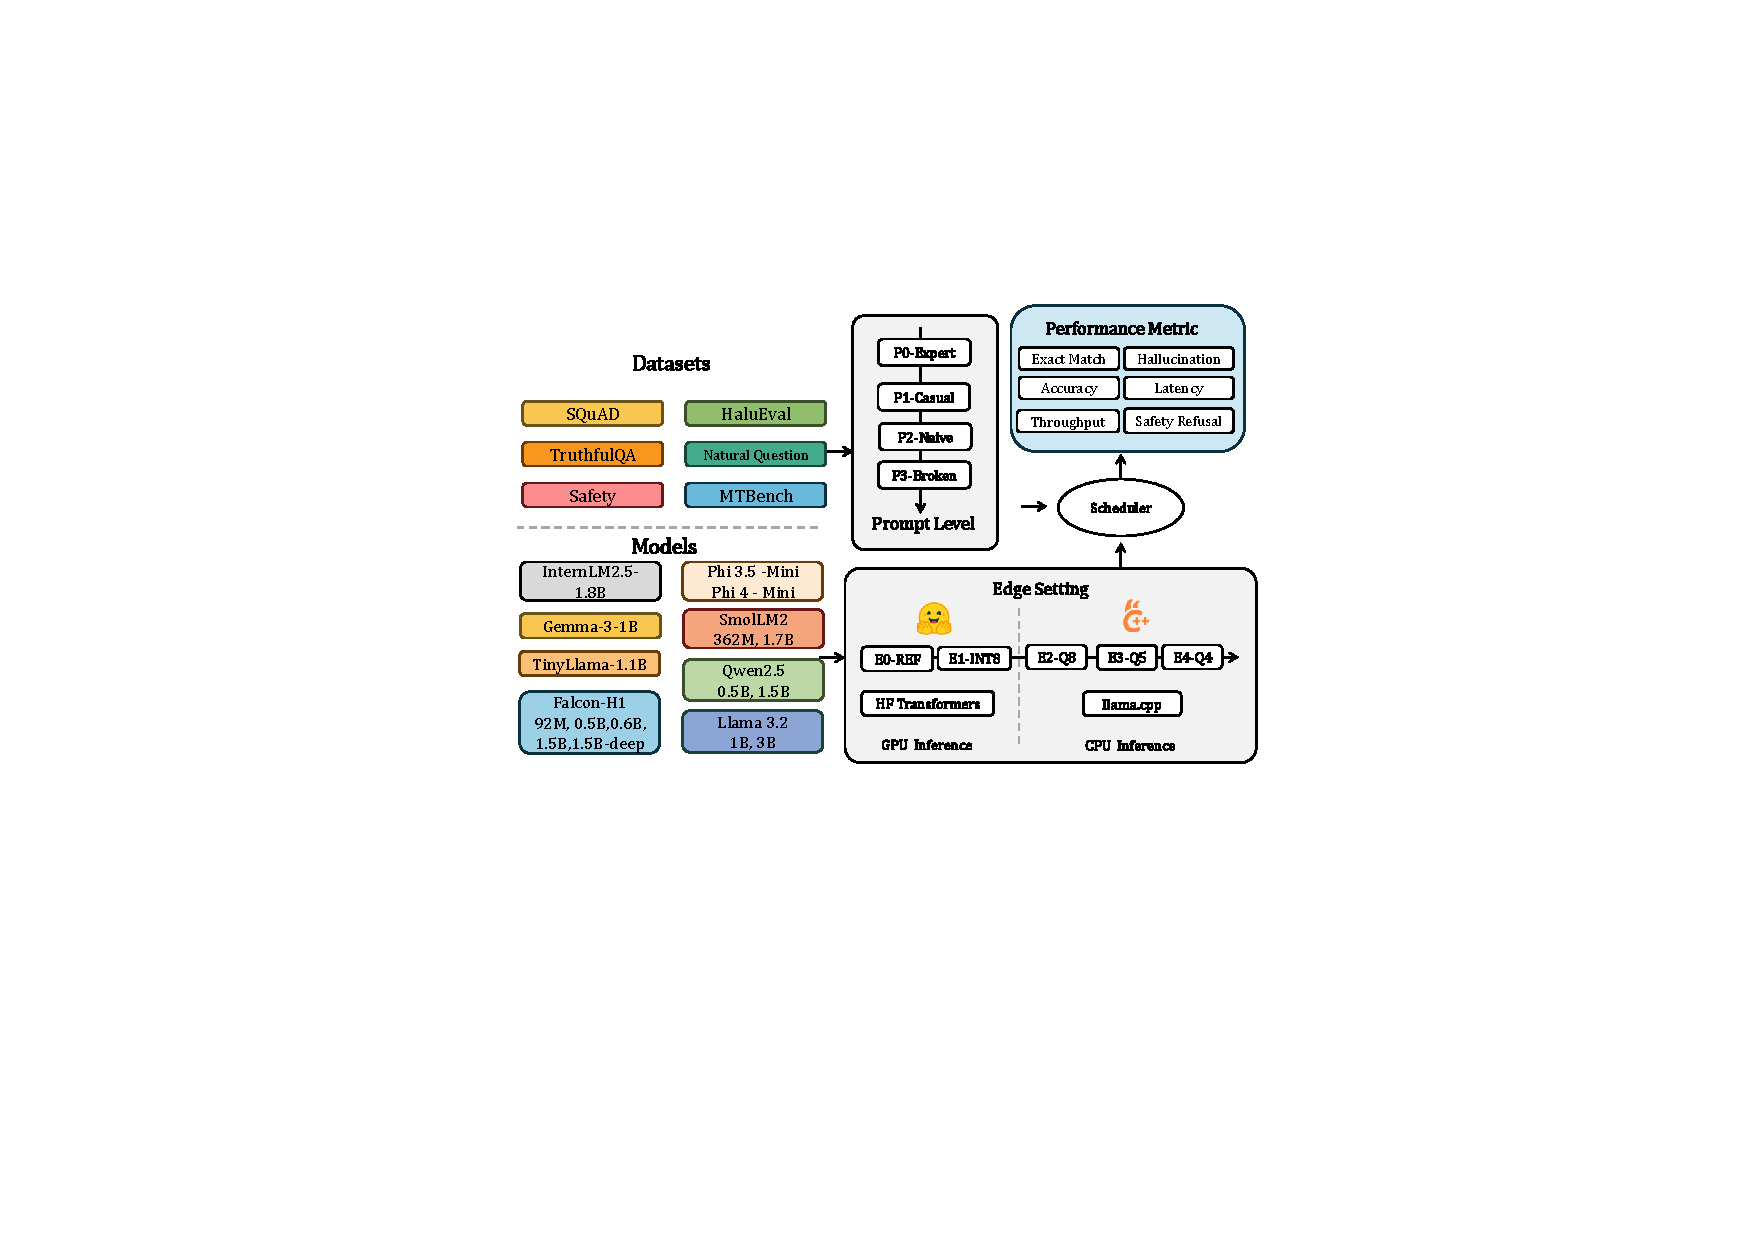
\includegraphics[width=\linewidth,height=0.24\textheight,keepaspectratio]{Figures/edgepipeline.pdf}
\caption{
Overview of PEEL, which evaluates sub-4B SLMs across prompt-quality
tiers (P0--P3) and edge settings (E0--E4), measuring accuracy, hallucination,
safety, quality, latency, and throughput.
}
    \label{fig:peel-framework}
\end{figure}

\section{Introduction}
\label{sec:intro}

Small language models (SLMs) are increasingly promoted as practical alternatives to cloud-scale large language models (LLMs). Their lower memory and compute requirements make local deployment feasible on laptops, mobile devices, and other resource-constrained hardware, supporting latency-sensitive, low-cost, and privacy-sensitive applications.

Yet local access changes what evaluation should measure. For ordinary users, practical value is not determined only by best-case benchmark scores under expert prompts and full-precision inference, but by what capability remains when prompts are vague, underspecified, or malformed and deployment relies on compressed local runtimes. Prior robustness work similarly treats worst-case or perturbed prompt performance as a reliability signal rather than nuisance variation~\cite{zhu2023promptrobust,ralpaca2024}. An SLM that appears capable under ideal prompts and server-class inference may therefore fail in the regime where it is meant to be useful.

We argue that SLM evaluation should report \emph{lower-bound reliability}: model behavior when user input quality and deployment quality degrade together. Existing evaluations cover parts of this space but rarely their interaction. General LLM benchmarks use standardized prompts and stable inference settings; edge benchmarks stress resource-constrained deployment but usually fix prompting; prompt-robustness studies perturb inputs while leaving the serving stack unchanged. This leaves limited evidence about ordinary users running SLMs locally.

We close this gap with \textbf{PEEL} (\textbf{P}rompt--\textbf{E}dge \textbf{E}valuation \textbf{L}adder), an automated benchmark for lower-bound SLM assessment. PEEL crosses four prompt-quality tiers, from expert instructions to broken ordinary-user prompts, with five edge-deployment settings, from full-precision GPU inference to low-bit local inference. It automates model/configuration selection, prompt construction, inference, offline scoring, and aggregation into reproducible run records across task accuracy, hallucination discrimination, safety behavior, instruction-following quality, latency, and throughput.

We evaluate 16 sub-4B SLMs across eight model families on extractive reading comprehension, open-domain QA, truthfulness, hallucination discrimination, safety, and multi-turn instruction following. Our central finding is that edge-deployed SLMs do not simply become weaker; their reliability becomes conditional on task format, prompt quality, runtime-interface fidelity, and scoring assumptions. On SQuAD~v2, model-averaged token-overlap F1 falls from roughly 30\% under expert prompts to \textbf{2--5\%} under broken prompts across edge settings, indicating near-total prompt-driven collapse in short-answer behavior. In contrast, TruthfulQA-MC1 changes only modestly from full precision to 4-bit inference under expert prompts after scoring artifacts are handled.

\paragraph{Contributions.}
We make the following contributions:
\begin{itemize}
\item \textbf{Automated PEEL framework.} We introduce an all-in-one benchmarking framework for lower-bound evaluation of edge-deployed SLMs, covering prompt construction, inference, scoring, and aggregation.

\item \textbf{Prompt--Edge Evaluation Ladder.} We define a two-axis protocol crossing four prompt-quality tiers with five edge-deployment settings, and evaluate 16 sub-4B SLMs across QA, truthfulness, hallucination, safety, and dialogue tasks.

\item \textbf{Prompt--edge reliability analysis.} We show that prompt degradation can dominate bit-width reduction for format-sensitive short-answer tasks, while multiple-choice truthfulness remains comparatively stable after scoring artifacts are handled.

\item \textbf{Falcon-H1 case study.} We analyze Falcon-H1, a recent SSM-hybrid SLM family, finding strong instruction-following performance while showing that prompt robustness is not architecture-exclusive.

\item \textbf{Reproducible artifacts.} We release prompts, deployment configurations, scoring scripts, per-run outputs, and machine-readable result grids for future lower-bound SLM evaluation.
\end{itemize}


\section{Related Work}
\label{sec:related}

\paragraph{Small language models, edge deployment, and quantization.}
Large language models have achieved strong performance across reasoning,
question answering, and instruction-following tasks, but their memory, compute,
and energy costs remain substantial for local or latency-sensitive deployment.
This has motivated compact SLM families such as TinyLlama~\cite{TinyLlama},
Phi~\cite{phi4}, Gemma~\cite{gemma2}, Qwen~\cite{qwen2025},
Llama-3.2~\cite{llama3}, and Falcon-H1~\cite{falconh1}. Falcon-H1 is especially
relevant because it is a recent SSM-Hybrid SLM family positioned for efficient
inference, yet its behavior under ordinary-user prompts and local-runtime
degradation has not been systematically characterized. In parallel,
edge-deployed SLM work studies model compression, efficient inference engines,
split execution, and hardware-aware deployment under latency, privacy,
bandwidth, and cost constraints~\cite{llm_edge,Mobileaibench,li2025palmbench}.
Post-training quantization methods such as GPTQ~\cite{gptq2022},
LLM.int8()~\cite{llmint8}, and lightweight runtimes such as
\texttt{llama.cpp}/GGUF~\cite{gguf} make local SLM inference increasingly
practical. However, quantization and runtime studies usually evaluate models
with fixed expert-style prompts, leaving open whether their conclusions hold
when users provide weak or underspecified instructions. 

\paragraph{Benchmarking and prompt robustness.}
General evaluation suites such as HELM~\cite{helm2022}, MMLU~\cite{mmlu2021},
SQuAD~v2~\cite{squad2}, Natural Questions~\cite{nqopen}, and
MT-Bench~\cite{mtbench2023} measure broad capability under standardized prompts
and stable inference stacks. SLM-oriented and edge benchmarks, including
JudgeBoard~\cite{smlbenchmark}, MobileAIBench~\cite{Mobileaibench}, and
PalmBench~\cite{li2025palmbench}, move closer to constrained deployment by
considering compact models, device compatibility, throughput, memory, energy,
or latency. These benchmarks are closest to our deployment motivation, but their
prompting protocols are typically fixed. Conversely, prompt-robustness studies
such as PromptBench~\cite{zhu2023promptrobust} and
RobustAlpacaEval~\cite{ralpaca2024} perturb prompt wording and formatting, but
generally keep the serving stack unchanged. PEEL differs by treating prompt
quality and deployment quality as a joint evaluation space: it asks whether a
model that survives quantization under expert prompts also remains reliable
under informal or underspecified prompts.

\paragraph{Trustworthiness and scoring fidelity.}
Trustworthiness is central to user-facing SLM deployment because local models
may have weaker instruction tuning and safety alignment while also bypassing
cloud-side safety layers. Prior benchmarks study truthfulness, hallucination,
toxicity, and unsafe instruction following through resources such as
TruthfulQA~\cite{truthfulqa}, HaluEval~\cite{halueval2023}, and safety-oriented
refusal tests. These evaluations are usually reported as task scores, assuming
that the model output can be parsed consistently across runtimes. PEEL
incorporates these dimensions, but also treats scoring fidelity as part of
benchmark design: local runtimes can alter output formatting, stop-token
behavior, prompt echoes, and chat-template handling, which can make parser
failures look like model failures. This motivates our audit-oriented evaluation
protocol, where benchmark scores are interpreted only after checking the runtime
and scoring assumptions behind them.

\section{\textbf{P}rompt--\textbf{E}dge \textbf{E}valuation \textbf{L}adder}
\label{sec:peel}

\subsection{Pipeline Overview}
\label{sec:pipeline}

Figure~\ref{fig:peel-framework} gives an overview of the
\textbf{P}rompt--\textbf{E}dge \textbf{E}valuation \textbf{L}adder (PEEL).
PEEL evaluates SLMs under two deployment-realistic sources of degradation:
weaker user prompts and more constrained local inference settings. The goal is
not to assign a single leaderboard score, but to expose whether failures are
driven by prompt quality, edge deployment, task format, or their interaction.

PEEL contains four stages. First, it selects compact model families and
user-facing benchmark tasks with different output contracts. Second, it
instantiates each task under a prompt-quality ladder, from expert benchmark
instructions to informal non-expert prompts. Third, it evaluates each model
under an edge-deployment ladder, from reference GPU inference to CPU-only GGUF
inference. Finally, it runs inference, normalizes runtime-specific outputs,
computes task metrics, and records efficiency measurements such as latency and
decode throughput. The result is a prompt--edge grid that allows direct
comparison across prompt tiers, deployment settings, model families, and task
types.

\begin{table}[t]
\centering

\label{tab:metrics}
\small
\begin{tabularx}{\columnwidth}{@{}p{0.24\columnwidth}p{0.23\columnwidth}X@{}}
\toprule
\textbf{Task} & \textbf{Dataset} & \textbf{Metric} \\
\midrule
Reading comp. & SQuAD v2 & Token-overlap F1 (primary); EM\\
Open QA & NQ-Open & Token-overlap F1 (primary); EM\\
Truthfulness & TruthfulQA-MC1 & Letter accuracy \\
Hallucination & HaluEval & Yes/No accuracy \\
Instruction following & MT-Bench & LLM-judge score\\
Safety behavior & Safety suite & ASR / refusal rates \\
Efficiency & All runs & Latency \& decode throughput \\
\bottomrule
\end{tabularx}
\caption{PEEL tasks and metrics. Reference-scored tasks use offline metrics after output normalization.}
\end{table}

\subsection{Tasks, Datasets, and Metrics}
\label{sec:tasks}

PEEL combines tasks with different output contracts: short answers, multiple-choice letters, binary judgments, refusal behavior, and open-ended dialogue. This lets us distinguish general capability loss from failures caused by output-format sensitivity or scoring interfaces.

For short-answer QA, we use SQuAD~v2~\citep{Rajpurkar2016SQuAD10} and NQ-Open~\citep{NQ_Google}. Because PEEL evaluates generative SLMs rather than extractive span models, we score generated answers with token-overlap F1 as the primary metric and exact match (EM) as a stricter secondary metric. SQuAD~v2 tests context-grounded answers, while NQ-Open tests parametric factual recall.

For factual reliability, we use TruthfulQA-MC1~\citep{truthfulqa} with generation-based multiple-choice letter selection, and HaluEval~\citep{Halueval_EMNLP23} as a binary hallucination judgment task. For safety, we evaluate unsafe prompts and benign refusal-sensitive prompts, reporting harmful-request attack success and benign over-refusal as separate failure modes.

Finally, we include MT-Bench~\citep{MTBenchArena_2023} for open-ended multi-turn instruction following. Because it uses LLM-judge scoring and a different output contract from reference-scored tasks, we report it separately rather than merging it into the F1/EM grids.
\subsection{Model Selection}
\label{sec:models}

PEEL focuses on a practical local-deployment regime: models from 90M to 3.8B
parameters (Table~\ref{tab:models}). This range is small enough to support
local inference after quantization, while still broad enough to compare model
families, parameter scales, and deployment sensitivity.

\begin{table}[t]
  \small
  \centering

  \begin{tabular}{@{}llc@{}}
    \toprule
    Model & Family \\
    \midrule
    Falcon-H1-Tiny-90M$^\ddagger$       & Falcon-H1~\citep{falconh1} \\
    Falcon-H1-0.5B$^\ddagger$           & Falcon-H1~\citep{falconh1} \\
    Falcon-H1-Tiny-R-0.6B$^\ddagger$    & Falcon-H1~\citep{falconh1}  \\
    Falcon-H1-1.5B$^\ddagger$           & Falcon-H1~\citep{falconh1} &\\
    Falcon-H1-1.5B-Deep$^\ddagger$      & Falcon-H1~\citep{falconh1} \\
    Gemma-3-1B                           & Gemma~\citep{gemmateam2025gemma3technicalreport} \\
    InternLM2.5-1.8B                     & InternLM~\citep{cai2024internlm2} \\
    Llama-3.2-1B                         & Llama~\citep{llama_3_2} \\
    Llama-3.2-3B                         & Llama~\citep{llama_3_2}  \\
    Phi-3.5-Mini                         & Phi~\citep{abdin2024phi3_2023}\\
    Phi-4-Mini                           & Phi~\citep{phi4}  \\
    Qwen2.5-0.5B                         & Qwen~\citep{qwen2025} \\
    Qwen2.5-1.5B                         & Qwen~\citep{qwen2025}  \\
    SmolLM2-360M                         & SmolLM~\citep{allal2025smollm2smolgoesbig} \\
    SmolLM2-1.7B                         & SmolLM~\citep{allal2025smollm2smolgoesbig} \\
    TinyLlama-1.1B                       & TinyLlama~\citep{tinyllama_2024}  \\
    \bottomrule
  \end{tabular}
    \caption{Models evaluated in PEEL.
  $^\ddagger$ denotes SSM-hybrid Falcon-H1 models.}
    \label{tab:models}
\end{table}

The model set has three roles. Falcon-H1~\citep{falconh1} is the primary family
of interest because it provides recent SSM-hybrid SLMs across several sizes.
Qwen~\citep{qwen2025}, Llama~\citep{llama_3_2},
Gemma~\citep{gemmateam2025gemma3technicalreport}, Phi~\citep{phi4},
SmolLM~\citep{allal2025smollm2smolgoesbig}, InternLM~\citep{cai2024internlm2},
and TinyLlama~\citep{tinyllama_2024} serve as recognizable SLM baselines. We do not use this model set to claim a universal winner; rather, we ask whether the same prompt and deployment perturbations produce consistent failure patterns across families.

\subsection{Edge Deployment Ladder}
\label{sec:edge}

PEEL evaluates each model under five named deployment settings, E0--E4.
These settings are deployment conditions rather than pure bit-width labels:
moving from reference GPU inference to local CPU inference changes not only
numeric precision, but also runtime implementation, quantization format,
chat-template handling, stop-token behavior, and resource budget.
\begin{itemize}
  \item \textbf{E0-REF}: BF16 Hugging Face inference on GPU.
  \item \textbf{E1-INT8}: INT8 Hugging Face inference with
  \texttt{bitsandbytes} on GPU.
  \item \textbf{E2-Q8}: Q8\_0 GGUF inference with \texttt{llama.cpp} on CPU.
  \item \textbf{E3-Q5}: Q5\_K\_M GGUF inference with \texttt{llama.cpp} on CPU.
  \item \textbf{E4-Q4}: Q4\_K\_M GGUF inference with \texttt{llama.cpp} on CPU.
\end{itemize}

E2--E4 use CPU-only inference to approximate local deployment without a
discrete GPU. The E0$\rightarrow$E1 contrast isolates GPU-side quantization,
while the E2$\rightarrow$E4 contrast varies quantization strength within the
same GGUF runtime. The E1$\rightarrow$E2 transition is intentionally treated as
a deployment transition rather than a pure quantization step, because it also
changes the inference runtime and serving interface.

\subsection{Prompt Quality Ladder}
\label{sec:prompt}

The second PEEL axis is prompt quality. We define four prompt tiers, P0--P3,
that preserve the underlying task while progressively weakening the user
instruction. Each tier keeps the question and required evidence, such as
context passages or answer options, but removes scaffolding or introduces
informal phrasing.

\begin{itemize}
  \item \textbf{P0 -- Expert}: Standard benchmark-style instruction with
  explicit task framing, labeled fields, and output constraints.
  \item \textbf{P1 -- Casual}: Grammatically correct natural-language prompt
  with reduced formatting and weaker output constraints.
  \item \textbf{P2 -- Naive}: Minimal prompt with little task framing; the
  model must infer the interaction contract.
\item \textbf{P3 -- Broken}: Informal, abbreviated, and syntactically weak
prompt resembling first-time or informal LLM use.
\end{itemize}

The prompt tiers are task-preserving rather than adversarial. We do not remove
the information needed to answer the question, inject contradictory content, or
change the label space. Thus, when performance drops under weaker prompts, the
failure indicates difficulty recovering the intended task contract rather than
absence of evidence.

\begin{table}[t]
  \small
  \centering

  \label{tab:prompts}
  \begin{tabular}{@{}lp{5.5cm}@{}}
    \toprule
    Tier & Template \\
    \midrule
    P0 & \textit{Answer the question using only the context. If the answer is
    not in the context, say `unanswerable'. Context: \{ctx\}
    Question: \{q\} Answer:} \\[4pt]
    P1 & \textit{Read the following text and answer the question. If the text
    doesn't have the answer, say so. Text: \{ctx\} Q: \{q\} A:} \\[4pt]
    P2 & \textit{\{q\} \textbackslash n\textbackslash n Here is some info:
    \{ctx\}} \\[4pt]
    P3 & \textit{pls help, \{q\}?? info: \{ctx\}} \\
    \bottomrule
  \end{tabular}
    \caption{SQuAD v2 prompt templates across PEEL prompt tiers.
  \texttt{\{ctx\}} and \texttt{\{q\}} are filled at run time.}
\end{table}

As a sanity check, we compare the PEEL tiers with real user prompts. We sample
50 single-turn English prompts from WildChat-1M~\citep{wildchat2024} and ask
three annotators to assign each prompt to the nearest PEEL tier. Two annotators
show moderate agreement (Cohen's $\kappa=0.51$, 70\% raw agreement), while the
third applies a systematically stricter mapping and tends to rate prompts one
tier lower (pairwise $\kappa\approx0.17$). We therefore treat the mapping as
approximate rather than calibrated. The useful observation is qualitative: most
sampled prompts fall below the expert tier, supporting P1--P3 as diagnostic
stress tests for non-expert interaction rather than as a population-calibrated
user model.

\subsection{Benchmark Automation and Reproducibility}

PEEL uses a unified registry for models, deployment settings, prompt tiers, and datasets. For each model--task--prompt--edge cell, it constructs the prompt, dispatches the appropriate inference backend, records runtime measurements, and applies offline task-specific scoring through the same execution interface. Generation and evaluation are separated. PEEL saves raw outputs before scoring, then computes metrics offline using deterministic parsers and runtime-aware normalization. This is important for local SLM runtimes, which may emit prompt echoes, end-of-text markers, or verbose continuations that otherwise create scoring artifacts. Each run stores its configuration, predictions, metrics, and summaries, enabling audit and rescoring. Experiments are launched through resumable scripts over the full prompt--edge grid. GPU settings cover reference and INT8 inference, while CPU GGUF settings represent local deployment. Full implementation details, run records, and reproducibility procedures are provided in the appendix and released artifacts.

\section{Results}
\label{sec:results}

We organize the results around five deployment-facing research questions. 
\subsection{RQ1: Does Edge Deployment Uniformly Degrade Accuracy?}
\label{sec:runtime-results}

Edge deployment clearly changes the systems profile, but it does not produce a
uniform accuracy collapse. Figure~\ref{fig:runtime-family} shows that the PEEL
edge ladder creates distinct efficiency regimes: GPU-backed Hugging Face
settings and CPU-backed \texttt{llama.cpp} settings differ substantially in
decode throughput and latency. E0/E1 provide the accelerated reference path,
while E2--E4 represent CPU-only local execution. This confirms that the edge
axis is a real deployment pressure. Accuracy, however, is task-dependent rather
than uniformly degraded: under P0, model-averaged SQuAD~v2 remains near
28--31\% token-overlap F1 across E0--E4 and TruthfulQA-MC1 changes modestly,
while NQ-Open shows a clearer E1$\rightarrow$E2 drop from 8.4\% to 3.6\%
token-overlap F1. Thus the edge ladder changes the runtime profile across the
benchmark, but damages accuracy mainly when the task and runtime interface are
sensitive to the deployment transition.
\begin{figure}[t]
    \centering
    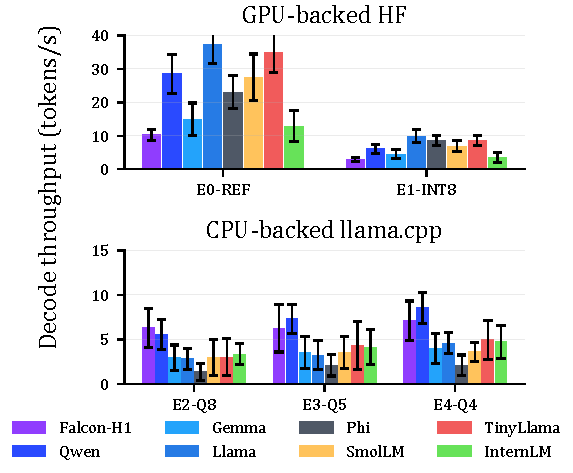
\includegraphics[width=0.9\linewidth]{fig4_2_throughput_B_family_average_ver2.pdf}
\caption{Family-level decode throughput across PEEL edge settings, separating GPU Hugging Face from CPU GGUF inference.}
    \label{fig:runtime-family}
\end{figure}

\subsection{RQ2: When Does Prompt Degradation Break SLMs?}
\label{sec:correctness-results}

\begin{figure}[t]
    \centering

    \begin{subfigure}[t]{0.9\linewidth}
        \centering
        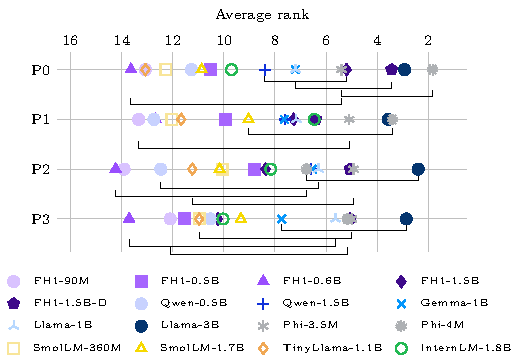
\includegraphics[width=\linewidth]
        {Figures/fig4_4_true2d_prompt_sequence_overall_correctness.pdf}
        \caption{Prompt sequence.}
        \label{fig:true2d_prompt_sequence}
    \end{subfigure}
    \hfill
    \begin{subfigure}[t]{0.9\linewidth}
        \centering
        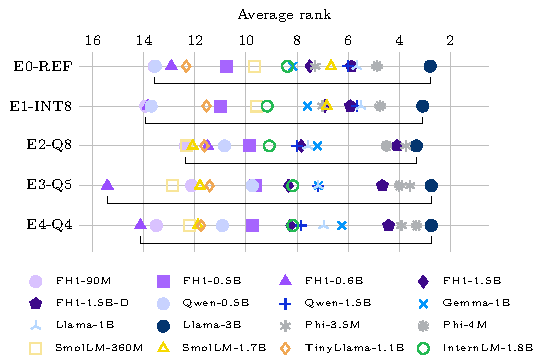
\includegraphics[width=\linewidth]
        {Figures/fig4_4_true2d_edge_sequence_overall_correctness.pdf}
        \caption{Edge sequence.}
        \label{fig:true2d_edge_sequence}
    \end{subfigure}
    \caption{Overall correctness under prompt and edge degradation sequences.}
    \label{fig:true2d_sequence_overall_correctness}
\end{figure}

Prompt degradation is most damaging when the task requires the model to recover an implicit output contract. Figure~\ref{fig:true2d_sequence_overall_correctness} aggregates SQuAD~v2, NQ-Open, and TruthfulQA-MC1 and compares model rankings along the prompt and edge axes. The prompt sequence separates model behavior more sharply than the edge sequence: several models change rank substantially from P0 to P3, whereas edge settings form broader groups with overlapping uncertainty. This does not mean that edge deployment is irrelevant; rather, weak prompts expose a distinct failure mode, especially when the prompt must specify the expected answer form.


\begin{table*}[t]
\centering
\small
\setlength{\tabcolsep}{2.2pt}
\renewcommand{\arraystretch}{0.92}

\begin{tabular}{rrrrr|rrrr|rrrr|rrrr|rrrr}
\toprule
\multirow{2}{*}{Model} & \multicolumn{4}{c}{E0-REF} & \multicolumn{4}{c}{E1-INT8} & \multicolumn{4}{c}{E2-Q8} & \multicolumn{4}{c}{E3-Q5} & \multicolumn{4}{c}{E4-Q4} \\
\cmidrule(lr){2-5} \cmidrule(lr){6-9} \cmidrule(lr){10-13} \cmidrule(lr){14-17} \cmidrule(lr){18-21}
 & P0 & P1 & P2 & P3 & P0 & P1 & P2 & P3 & P0 & P1 & P2 & P3 & P0 & P1 & P2 & P3 & P0 & P1 & P2 & P3 \\
\midrule
Falcon-H1-Tiny-90M& \cellcolor[HTML]{F9D2CC}21.5 & \cellcolor[HTML]{F8CCCC}17.5 & \cellcolor[HTML]{FAD6CC}24.0 & \cellcolor[HTML]{FBDECC}29.5 & \cellcolor[HTML]{F9CFCC}19.0 & \cellcolor[HTML]{F8CDCC}17.5 & \cellcolor[HTML]{F9D3CC}21.5 & \cellcolor[HTML]{FBDACC}26.5 & \cellcolor[HTML]{FAD5CC}25.0 & \cellcolor[HTML]{F9D2CC}23.0 & \cellcolor[HTML]{F8CECC}20.5 & \cellcolor[HTML]{F9CFCC}21.0 & \cellcolor[HTML]{F9D2CC}23.0 & \cellcolor[HTML]{F9D2CC}23.0 & \cellcolor[HTML]{F8CDCC}20.0 & \cellcolor[HTML]{F9CFCC}21.5 & \cellcolor[HTML]{F8CDCC}19.5 & \cellcolor[HTML]{F8CECC}20.5 & \cellcolor[HTML]{F8CCCC}19.0 & \cellcolor[HTML]{F9D3CC}23.5 \\
Falcon-H1-0.5B& \cellcolor[HTML]{FEECCC}38.5 & \cellcolor[HTML]{FBDFCC}30.0 & \cellcolor[HTML]{FCE2CC}32.0 & \cellcolor[HTML]{FBDDCC}28.5 & \cellcolor[HTML]{FFF0CC}40.5 & \cellcolor[HTML]{FCE4CC}33.0 & \cellcolor[HTML]{FCE1CC}31.0 & \cellcolor[HTML]{FBDDCC}28.0 & \cellcolor[HTML]{FFF0CC}43.0 & \cellcolor[HTML]{F9D0CC}21.5 & \cellcolor[HTML]{FFF1CC}43.5 & \cellcolor[HTML]{F9D1CC}22.5 & \cellcolor[HTML]{FCF1CC}44.0 & \cellcolor[HTML]{F9D2CC}23.0 & \cellcolor[HTML]{FFF0CC}41.5 & \cellcolor[HTML]{F8CCCC}19.5 & \cellcolor[HTML]{FFF0CC}40.5 & \cellcolor[HTML]{F9D1CC}22.0 & \cellcolor[HTML]{FFF1CC}41.5 & \cellcolor[HTML]{F9D0CC}21.5 \\
Falcon-H1-Tiny-R-0.6B & \cellcolor[HTML]{F9D3CC}22.0 & \cellcolor[HTML]{F9D2CC}21.5 & \cellcolor[HTML]{F9D4CC}22.5 & \cellcolor[HTML]{F9D1CC}21.0 & \cellcolor[HTML]{F9D4CC}22.0 & \cellcolor[HTML]{FAD5CC}23.0 & \cellcolor[HTML]{F9D2CC}21.0 & \cellcolor[HTML]{F9D2CC}21.0 & \cellcolor[HTML]{FBDCCC}29.5 & \cellcolor[HTML]{FAD4CC}24.5 & \cellcolor[HTML]{F8CECC}20.0 & \cellcolor[HTML]{F9D2CC}23.0 & \cellcolor[HTML]{F8CDCC}20.0 & \cellcolor[HTML]{F9D0CC}22.0 & \cellcolor[HTML]{F8CCCC}19.5 & \cellcolor[HTML]{F8CECC}20.5 & \cellcolor[HTML]{FAD8CC}26.5 & \cellcolor[HTML]{FAD7CC}25.5 & \cellcolor[HTML]{F8CCCC}19.0 & \cellcolor[HTML]{FAD5CC}24.5 \\
Falcon-H1-1.5B & \cellcolor[HTML]{E2ECCC}57.0 & \cellcolor[HTML]{E1ECCC}57.5 & \cellcolor[HTML]{FFF1CC}42.0 & \cellcolor[HTML]{F7F1CC}46.5 & \cellcolor[HTML]{E1ECCC}56.5 & \cellcolor[HTML]{DAEBCC}60.0 & \cellcolor[HTML]{FEEFCC}40.0 & \cellcolor[HTML]{F7F0CC}46.0 & \cellcolor[HTML]{FAF1CC}46.5 & \cellcolor[HTML]{FAD5CC}25.0 & \cellcolor[HTML]{FCE4CC}35.0 & \cellcolor[HTML]{FAD6CC}25.5 & \cellcolor[HTML]{FBF1CC}44.5 & \cellcolor[HTML]{F9D0CC}22.0 & \cellcolor[HTML]{FCE4CC}34.0 & \cellcolor[HTML]{FAD4CC}24.5 & \cellcolor[HTML]{FDF2CC}43.0 & \cellcolor[HTML]{FAD5CC}24.5 & \cellcolor[HTML]{FCE3CC}33.0 & \cellcolor[HTML]{FAD4CC}24.0 \\
 Falcon-H1-1.5B-Deep & \cellcolor[HTML]{D5EACC}63.5 & \cellcolor[HTML]{CEE8CC}67.0 & \cellcolor[HTML]{DBEBCC}60.5 & \cellcolor[HTML]{DBEBCC}60.5 & \cellcolor[HTML]{D6EACC}62.0 & \cellcolor[HTML]{CFE9CC}65.5 & \cellcolor[HTML]{DDEBCC}58.5 & \cellcolor[HTML]{D5EACC}62.5 & \cellcolor[HTML]{DCEBCC}61.5 & \cellcolor[HTML]{FEEECC}41.5 & \cellcolor[HTML]{EAEECC}54.5 & \cellcolor[HTML]{F2F0CC}50.5 & \cellcolor[HTML]{D6EACC}61.0 & \cellcolor[HTML]{EFEFCC}49.5 & \cellcolor[HTML]{D8EACC}60.0 & \cellcolor[HTML]{F6F0CC}46.5 & \cellcolor[HTML]{D6EACC}60.5 & \cellcolor[HTML]{E7EDCC}53.0 & \cellcolor[HTML]{DCEBCC}58.0 & \cellcolor[HTML]{EAEECC}51.5 \\
Qwen-0.5B & \cellcolor[HTML]{FAD6CC}24.0 & \cellcolor[HTML]{F9D3CC}22.0 & \cellcolor[HTML]{F9D2CC}21.5 & \cellcolor[HTML]{F9D3CC}22.0 & \cellcolor[HTML]{F9D4CC}22.0 & \cellcolor[HTML]{FAD6CC}23.5 & \cellcolor[HTML]{F9D4CC}22.0 & \cellcolor[HTML]{FAD7CC}24.5 & \cellcolor[HTML]{FBDDCC}30.0 & \cellcolor[HTML]{F9D1CC}22.0 & \cellcolor[HTML]{F9D0CC}21.5 & \cellcolor[HTML]{F9D4CC}24.0 & \cellcolor[HTML]{FAD8CC}26.5 & \cellcolor[HTML]{FAD8CC}26.5 & \cellcolor[HTML]{FAD4CC}24.5 & \cellcolor[HTML]{FBDACC}28.0 & \cellcolor[HTML]{FBDACC}27.5 & \cellcolor[HTML]{F9CFCC}21.0 & \cellcolor[HTML]{F9D3CC}23.0 & \cellcolor[HTML]{FAD6CC}25.0 \\
Qwen-1.5B & \cellcolor[HTML]{ECEECC}52.0 & \cellcolor[HTML]{F0EFCC}50.0 & \cellcolor[HTML]{FAF1CC}45.0 & \cellcolor[HTML]{FEEFCC}40.5 & \cellcolor[HTML]{ECEECC}51.5 & \cellcolor[HTML]{F2EFCC}48.5 & \cellcolor[HTML]{FEF2CC}42.5 & \cellcolor[HTML]{FEEDCC}39.0 & \cellcolor[HTML]{ECEECC}53.5 & \cellcolor[HTML]{FDE5CC}35.5 & \cellcolor[HTML]{F9D3CC}23.5 & \cellcolor[HTML]{FBDDCC}30.0 & \cellcolor[HTML]{E9EECC}52.5 & \cellcolor[HTML]{FDE8CC}36.5 & \cellcolor[HTML]{FAD6CC}25.5 & \cellcolor[HTML]{FDE6CC}35.0 & \cellcolor[HTML]{E1ECCC}55.5 & \cellcolor[HTML]{FAD8CC}26.0 & \cellcolor[HTML]{FBDDCC}29.5 & \cellcolor[HTML]{FCE1CC}31.5 \\
Gemma-1B & \cellcolor[HTML]{FAD8CC}25.5 & \cellcolor[HTML]{FAD8CC}25.5 & \cellcolor[HTML]{FAD9CC}26.0 & \cellcolor[HTML]{FAD8CC}25.5 & \cellcolor[HTML]{FBDECC}29.0 & \cellcolor[HTML]{FBDBCC}27.0 & \cellcolor[HTML]{FBDACC}26.5 & \cellcolor[HTML]{FBDACC}26.0 & \cellcolor[HTML]{F9D1CC}22.5 & \cellcolor[HTML]{F9D0CC}21.5 & \cellcolor[HTML]{F8CECC}20.5 & \cellcolor[HTML]{F9CFCC}21.0 & \cellcolor[HTML]{FAD4CC}24.5 & \cellcolor[HTML]{F8CECC}21.0 & \cellcolor[HTML]{F9CFCC}21.5 & \cellcolor[HTML]{F9CFCC}21.5 & \cellcolor[HTML]{FBDDCC}29.0 & \cellcolor[HTML]{F8CECC}20.5 & \cellcolor[HTML]{F9D2CC}22.5 & \cellcolor[HTML]{FAD4CC}24.0 \\
Llama-1B & \cellcolor[HTML]{FDE5CC}34.0 & \cellcolor[HTML]{FEEECC}40.0 & \cellcolor[HTML]{FDE6CC}34.5 & \cellcolor[HTML]{FCE3CC}32.5 & \cellcolor[HTML]{FDE8CC}35.5 & \cellcolor[HTML]{FFF2CC}42.0 & \cellcolor[HTML]{FDE8CC}35.5 & \cellcolor[HTML]{FCE0CC}30.0 & \cellcolor[HTML]{FAD7CC}26.0 & \cellcolor[HTML]{F9D1CC}22.0 & \cellcolor[HTML]{FCE1CC}33.0 & \cellcolor[HTML]{FCE0CC}32.5 & \cellcolor[HTML]{FBDCCC}29.0 & \cellcolor[HTML]{F9CFCC}21.5 & \cellcolor[HTML]{FCE1CC}32.0 & \cellcolor[HTML]{FAD8CC}26.5 & \cellcolor[HTML]{FCE0CC}31.0 & \cellcolor[HTML]{F9D1CC}22.0 & \cellcolor[HTML]{FCE3CC}33.0 & \cellcolor[HTML]{F9D1CC}22.0 \\
Llama-3B & \cellcolor[HTML]{DEECCC}59.0 & \cellcolor[HTML]{CCE8CC}68.0 & \cellcolor[HTML]{DEECCC}59.0 & \cellcolor[HTML]{E5EDCC}55.5 & \cellcolor[HTML]{E0ECCC}57.0 & \cellcolor[HTML]{D1E9CC}64.5 & \cellcolor[HTML]{DEECCC}58.0 & \cellcolor[HTML]{E7EDCC}54.0 & \cellcolor[HTML]{DDEBCC}61.0 & \cellcolor[HTML]{FBF1CC}46.0 & \cellcolor[HTML]{FFF0CC}43.0 & \cellcolor[HTML]{FDE6CC}36.0 & \cellcolor[HTML]{D6EACC}61.0 & \cellcolor[HTML]{F6F0CC}46.5 & \cellcolor[HTML]{F3F0CC}48.0 & \cellcolor[HTML]{FEEBCC}38.5 & \cellcolor[HTML]{DCEBCC}58.0 & \cellcolor[HTML]{F6F0CC}46.0 & \cellcolor[HTML]{FDF2CC}43.0 & \cellcolor[HTML]{FEECCC}38.5 \\
Phi-3.5Mini & \cellcolor[HTML]{CEE8CC}67.0 & \cellcolor[HTML]{CCE8CC}68.0 & \cellcolor[HTML]{E6EDCC}55.0 & \cellcolor[HTML]{D5EACC}63.5 & \cellcolor[HTML]{CFE9CC}65.5 & \cellcolor[HTML]{CCE8CC}67.0 & \cellcolor[HTML]{EFEFCC}50.0 & \cellcolor[HTML]{D2E9CC}64.0 & \cellcolor[HTML]{D1E9CC}67.0 & \cellcolor[HTML]{FDF2CC}45.0 & \cellcolor[HTML]{FEEFCC}42.0 & \cellcolor[HTML]{FDE7CC}37.0 & \cellcolor[HTML]{D6EACC}61.0 & \cellcolor[HTML]{DCEBCC}58.5 & \cellcolor[HTML]{E1ECCC}56.0 & \cellcolor[HTML]{D9EBCC}59.5 & \cellcolor[HTML]{CCE8CC}65.0 & \cellcolor[HTML]{D5EACC}61.0 & \cellcolor[HTML]{EDEFCC}50.0 & \cellcolor[HTML]{DEEBCC}57.0 \\
Phi-4Mini & \cellcolor[HTML]{D5EACC}63.5 & \cellcolor[HTML]{CFE9CC}66.5 & \cellcolor[HTML]{D6EACC}63.0 & \cellcolor[HTML]{D3E9CC}64.5 & \cellcolor[HTML]{D3E9CC}63.5 & \cellcolor[HTML]{CEE8CC}66.0 & \cellcolor[HTML]{D2E9CC}64.0 & \cellcolor[HTML]{CFE9CC}65.5 & \cellcolor[HTML]{CCE8CC}69.5 & \cellcolor[HTML]{ECEECC}53.5 & \cellcolor[HTML]{FEEDCC}41.0 & \cellcolor[HTML]{F1EFCC}51.0 & \cellcolor[HTML]{CCE8CC}65.5 & \cellcolor[HTML]{E8EDCC}53.0 & \cellcolor[HTML]{FBF1CC}44.5 & \cellcolor[HTML]{FFF1CC}42.0 & \cellcolor[HTML]{D3E9CC}62.0 & \cellcolor[HTML]{F7F0CC}45.5 & \cellcolor[HTML]{F7F0CC}45.5 & \cellcolor[HTML]{E8EDCC}52.5 \\
SmolLM-360M & \cellcolor[HTML]{FAD5CC}23.5 & \cellcolor[HTML]{F8CECC}18.5 & \cellcolor[HTML]{F8CECC}19.0 & \cellcolor[HTML]{F8CECC}18.5 & \cellcolor[HTML]{FAD5CC}23.0 & \cellcolor[HTML]{F9D0CC}19.5 & \cellcolor[HTML]{FAD6CC}23.5 & \cellcolor[HTML]{F9D4CC}22.0 & \cellcolor[HTML]{F8CECC}20.5 & \cellcolor[HTML]{F9D1CC}22.5 & \cellcolor[HTML]{F9CFCC}21.0 & \cellcolor[HTML]{F9CFCC}21.0 & \cellcolor[HTML]{F8CDCC}20.0 & \cellcolor[HTML]{F8CECC}21.0 & \cellcolor[HTML]{F9D1CC}22.5 & \cellcolor[HTML]{F9D0CC}22.0 & \cellcolor[HTML]{F8CECC}20.0 & \cellcolor[HTML]{F9D1CC}22.0 & \cellcolor[HTML]{F8CECC}20.0 & \cellcolor[HTML]{F8CECC}20.0 \\
SmolLM-1.7B & \cellcolor[HTML]{FAD6CC}24.0 & \cellcolor[HTML]{FDE9CC}36.5 & \cellcolor[HTML]{FBDACC}27.0 & \cellcolor[HTML]{FCE3CC}32.5 & \cellcolor[HTML]{FAD7CC}24.0 & \cellcolor[HTML]{FDE6CC}34.0 & \cellcolor[HTML]{FAD7CC}24.5 & \cellcolor[HTML]{FCDFCC}29.5 & \cellcolor[HTML]{F9D1CC}22.0 & \cellcolor[HTML]{F9D1CC}22.0 & \cellcolor[HTML]{F8CCCC}19.0 & \cellcolor[HTML]{F9D1CC}22.0 & \cellcolor[HTML]{F8CDCC}20.0 & \cellcolor[HTML]{F9D0CC}22.0 & \cellcolor[HTML]{F8CDCC}20.0 & \cellcolor[HTML]{F8CECC}21.0 & \cellcolor[HTML]{F9CFCC}21.0 & \cellcolor[HTML]{F9D2CC}22.5 & \cellcolor[HTML]{F9CFCC}21.0 & \cellcolor[HTML]{F8CECC}20.0 \\
TinyLlama-1.1B & \cellcolor[HTML]{F9D0CC}20.0 & \cellcolor[HTML]{F9D0CC}20.0 & \cellcolor[HTML]{F8CECC}18.5 & \cellcolor[HTML]{FAD4CC}23.0 & \cellcolor[HTML]{F9D1CC}20.0 & \cellcolor[HTML]{FAD7CC}24.0 & \cellcolor[HTML]{F8CCCC}17.0 & \cellcolor[HTML]{F9D2CC}21.0 & \cellcolor[HTML]{FAD4CC}24.5 & \cellcolor[HTML]{F8CECC}20.0 & \cellcolor[HTML]{F8CECC}20.5 & \cellcolor[HTML]{F9D0CC}21.5 & \cellcolor[HTML]{F9CFCC}21.5 & \cellcolor[HTML]{F8CCCC}19.5 & \cellcolor[HTML]{F9D2CC}23.0 & \cellcolor[HTML]{F9D3CC}23.5 & \cellcolor[HTML]{F9D2CC}22.5 & \cellcolor[HTML]{F8CECC}20.0 & \cellcolor[HTML]{FBDACC}27.5 & \cellcolor[HTML]{F9D2CC}22.5 \\
InternLM-1.8B & \cellcolor[HTML]{FFF1CC}42.0 & \cellcolor[HTML]{FEEECC}40.0 & \cellcolor[HTML]{FEEACC}37.5 & \cellcolor[HTML]{FDE7CC}35.5 & \cellcolor[HTML]{FFF2CC}42.0 & \cellcolor[HTML]{FEEECC}39.5 & \cellcolor[HTML]{FEECCC}38.0 & \cellcolor[HTML]{FDEACC}36.5 & \cellcolor[HTML]{FEEACC}39.0 & \cellcolor[HTML]{FDE6CC}36.0 & \cellcolor[HTML]{FCE3CC}34.5 & \cellcolor[HTML]{FBDDCC}30.5 & \cellcolor[HTML]{FEEFCC}40.5 & \cellcolor[HTML]{FEEECC}40.0 & \cellcolor[HTML]{FDE6CC}35.0 & \cellcolor[HTML]{FCE1CC}32.0 & \cellcolor[HTML]{FDE7CC}35.5 & \cellcolor[HTML]{FCE0CC}31.0 & \cellcolor[HTML]{FFF0CC}40.5 & \cellcolor[HTML]{FDE5CC}34.0 \\
\bottomrule
\end{tabular}%
\caption{TruthfulQA-MC1 accuracy (\%) across edge settings and prompt tiers. Cell color is normalized within each edge-setting block; greener cells indicate higher accuracy.}
\label{tab:truthfulqa-mc1-correctness-grid}
\end{table*}


\begin{table}[t]
\centering

\setlength{\tabcolsep}{2.4pt}
\renewcommand{\arraystretch}{0.92}
\begin{tabular}{rcccc|cccc}
\toprule
Edge & \multicolumn{4}{c}{SQuAD v2} & \multicolumn{4}{c}{NQ-Open} \\
\cmidrule(lr){2-5} \cmidrule(lr){6-9}
 & P0 & P1 & P2 & P3 & P0 & P1 & P2 & P3 \\
\midrule
E0-REF & \cellcolor[HTML]{D9EAD3}30.5 & \cellcolor[HTML]{FEF2CC}16.8 & \cellcolor[HTML]{F7D5CC}5.6 & \cellcolor[HTML]{F6D3CC}4.7 & \cellcolor[HTML]{DBEAD3}8.2 & \cellcolor[HTML]{F9DECC}3.2 & \cellcolor[HTML]{F9DCCC}3.0 & \cellcolor[HTML]{F9DDCC}3.1 \\
E1-INT8 & \cellcolor[HTML]{D9EAD3}30.4 & \cellcolor[HTML]{FEF2CC}16.6 & \cellcolor[HTML]{F7D5CC}5.6 & \cellcolor[HTML]{F6D3CC}4.7 & \cellcolor[HTML]{D9EAD3}8.4 & \cellcolor[HTML]{F9DDCC}3.1 & \cellcolor[HTML]{F8DBCC}3.0 & \cellcolor[HTML]{F8DCCC}3.0 \\
E2-Q8 & \cellcolor[HTML]{D9EAD3}30.5 & \cellcolor[HTML]{F2EFCE}21.1 & \cellcolor[HTML]{F5CFCC}3.4 & \cellcolor[HTML]{F4CDCC}2.4 & \cellcolor[HTML]{FBE3CC}3.6 & \cellcolor[HTML]{F5CFCC}1.9 & \cellcolor[HTML]{F5CFCC}1.8 & \cellcolor[HTML]{F4CDCC}1.7 \\
E3-Q5 & \cellcolor[HTML]{DBEAD3}29.7 & \cellcolor[HTML]{F7F0CE}19.4 & \cellcolor[HTML]{F5CECC}3.1 & \cellcolor[HTML]{F4CCCC}2.2 & \cellcolor[HTML]{FAE2CC}3.5 & \cellcolor[HTML]{F5CECC}1.8 & \cellcolor[HTML]{F4CECC}1.8 & \cellcolor[HTML]{F4CDCC}1.7 \\
E4-Q4 & \cellcolor[HTML]{E0ECD2}27.8 & \cellcolor[HTML]{F8F1CD}18.8 & \cellcolor[HTML]{F5CECC}3.0 & \cellcolor[HTML]{F4CCCC}2.3 & \cellcolor[HTML]{F9DFCC}3.3 & \cellcolor[HTML]{F4CDCC}1.7 & \cellcolor[HTML]{F4CDCC}1.7 & \cellcolor[HTML]{F4CCCC}1.6 \\
\bottomrule
\end{tabular}%
\caption{Token-overlap F1 (\%) for short-answer QA, averaged across models by dataset. Strict exact-match results are reported in the supplementary material.}
\label{tab:short-answer-edge-prompt-em}
\end{table}


Table~\ref{tab:short-answer-edge-prompt-em} shows where the break happens. For SQuAD~v2, token-overlap F1 remains close to 28--31\% under P0 across all edge settings, but drops to 2--5\% under P3. This is a near-total task-contract collapse: the weak prompt no longer reliably elicits the short span-like answer that overlaps the gold reference. NQ-Open is harder overall and shows an additional deployment boundary: P0 F1 is 8.2--8.4\% under E0/E1, but falls to 3.3--3.6\% under GGUF-based edge settings. Strict exact match is lower throughout (SQuAD $\approx$21\% at P0 and $\approx$0\% at P3; NQ-Open $\leq$2\% even at P0; see supplementary material), so these short-answer scores should be read as answer overlap rather than strict-format capability. Thus SQuAD primarily exposes prompt-contract fragility, while NQ-Open combines recall-like knowledge demand, runtime-interface sensitivity, and prompt degradation.

\paragraph{Prompt$\times$edge interaction.}
We next ask whether the edge ladder amplifies prompt sensitivity, rather than the two axes acting independently. For each task, we compute three model-level quantities: the prompt effect (P0$-$P3, averaged over edge settings), the edge effect (E0$-$E4, averaged over prompt tiers), and the interaction, defined as the prompt effect at E4 minus the prompt effect at E0. Positive interaction values indicate that edge deployment amplifies prompt sensitivity. We report 95\% bootstrap confidence intervals over 16 models using 10{,}000 resamples.

The result is task-dependent. For SQuAD~v2, the prompt effect is large ($26.3$ F1 pts, CI $[19.6, 32.9]$), while the edge effect ($1.4$, CI $[-2.0, 4.9]$) and interaction ($-0.2$, CI $[-8.3, 7.6]$) are indistinguishable from zero. Prompt degradation therefore dominates SQuAD and does so additively, independent of bit-width. For NQ-Open, the interaction is negative ($-3.4$, CI $[-5.5, -1.7]$), because edge deployment pushes answer overlap toward the floor and leaves less room for prompts to matter. Only TruthfulQA-MC1 shows a positive interaction ($+5.8$ pts, CI $[3.2, 8.2]$): its prompt effect grows from $2.1$ at E0 to $7.8$ at E4, so here the edge setting genuinely amplifies prompt sensitivity. We therefore do not claim a general multiplicative interaction. The headline short-answer collapse is a dominant, edge-independent prompt effect, while multiple-choice truthfulness is the clearest case where prompt and deployment degradation compound.

\subsection{RQ3: Are All Tasks Equally Fragile?}
\label{sec:task-fragility-results}

PEEL shows that task format mediates robustness. TruthfulQA-MC1 behaves
differently from short-answer QA because the model selects from explicit answer
options, making the output contract less dependent on span extraction, answer
formatting, or exact surface form. Table~\ref{tab:truthfulqa-mc1-correctness-grid}
therefore provides a multiple-choice counterpoint to the short-answer results.
Accuracy varies substantially across model families, but there is no universal
P3 collapse comparable to SQuAD~v2 or NQ-Open. Several models still exhibit
prompt sensitivity under the more constrained E2--E4 settings: Falcon-H1-1.5B,
Qwen-1.5B, and Llama-3B decline from P0 to weaker prompt tiers, while
Falcon-H1-0.5B displays large but non-monotonic fluctuations. These results
indicate that prompt and edge degradation interact in a model- and
task-dependent manner rather than producing a single universal failure pattern.



\begin{figure}[t]
    \centering
    \begin{subfigure}[t]{0.49\textwidth}
        \centering
        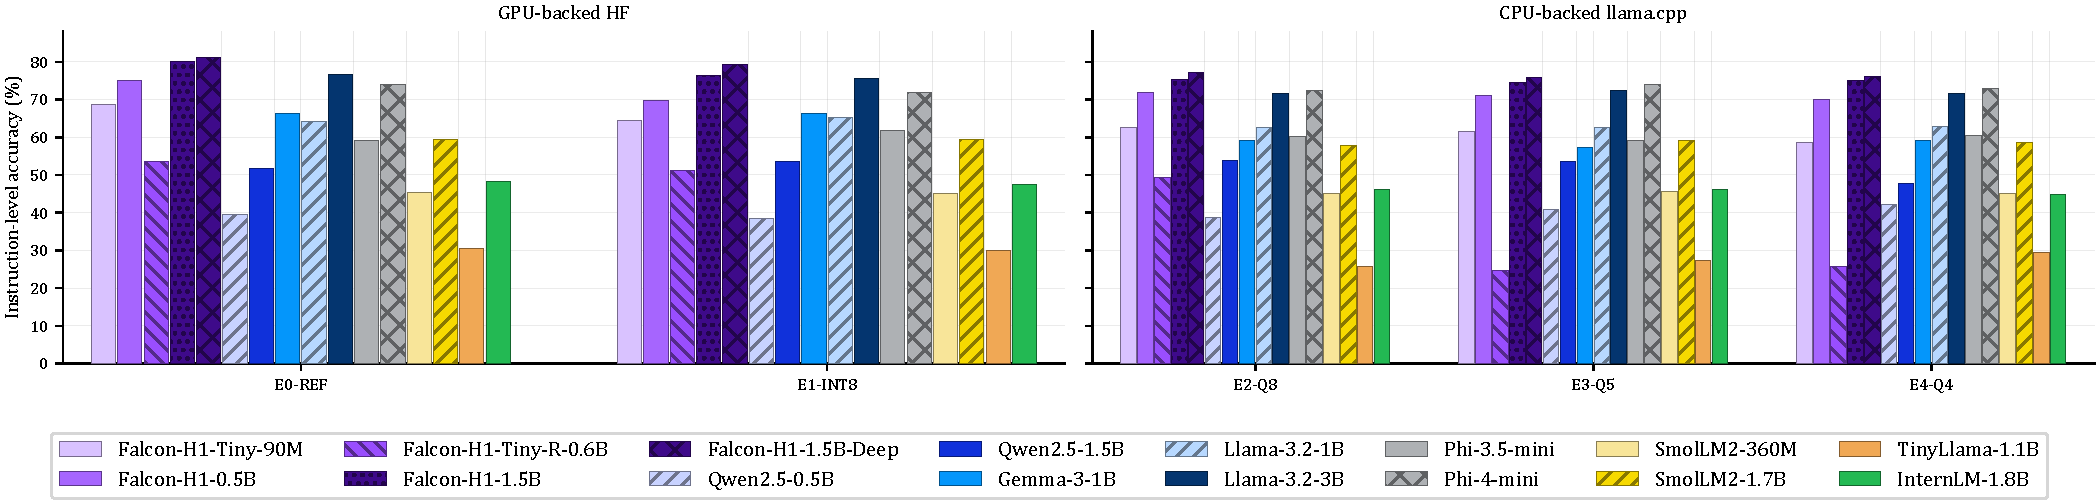
\includegraphics[width=\linewidth]{Figures/fig4_5_ifeval_instr_acc_model_bars.pdf}
        \caption{Instruction-level accuracy.}
        \label{fig:ifeval-instr-acc}
    \end{subfigure}
    \hfill
    \begin{subfigure}[t]{0.49\textwidth}
        \centering
        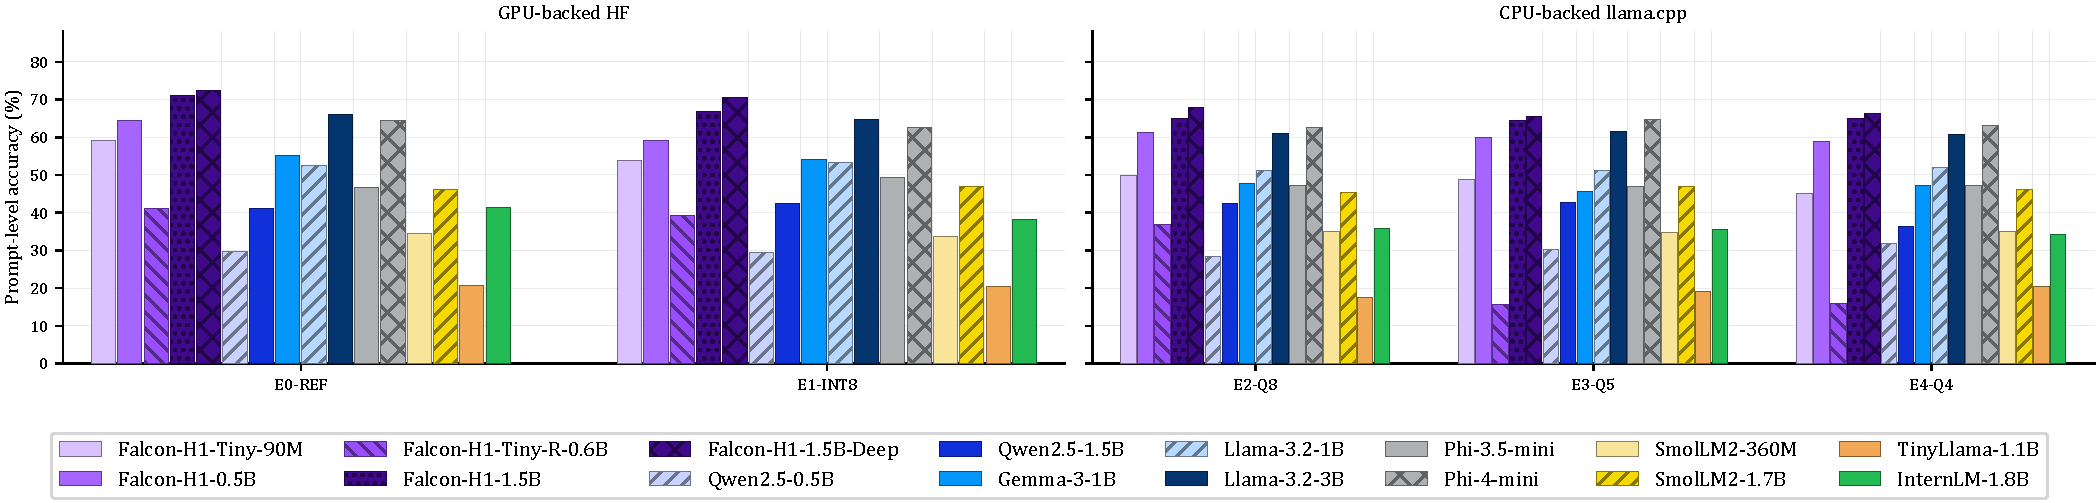
\includegraphics[width=\linewidth]{Figures/fig4_5_ifeval_prompt_acc_model_bars.pdf}
        \caption{Prompt-level accuracy.}
        \label{fig:ifeval-prompt-acc}
    \end{subfigure}
\caption{IFEval compliance under P0. \emph{prompt\_acc} is an IFEval metric, not a PEEL prompt tier.}
    \label{fig:ifeval-compliance-bars}
\end{figure}


\paragraph{Rule-based compliance and hallucination.}
IFEval and HaluEval evaluate rule-following and binary hallucination
classification rather than reference-string matching. Both tasks are evaluated
under P0 only. IFEval reports instruction-level and prompt-level compliance, while HaluEval measures
whether a model can identify hallucinated responses.

The IFEval results show that differences between model families are generally
larger than the changes across edge settings, with most models maintaining
similar relative performance under quantization. HaluEval-General exhibits a
clearer edge effect for several models, whereas HaluEval-QA varies less
consistently across edge settings. Overall, rule-based performance is primarily
model-dependent, although edge degradation affects some models more strongly
than others. These tasks broaden the task-fragility picture: not every metric
is a prompt-tier metric, and not every output contract fails in the same way.
Detailed model-level HaluEval results are provided in
Appendix~\ref{app:halueval-results}.




\begin{figure}[t]
    \centering
    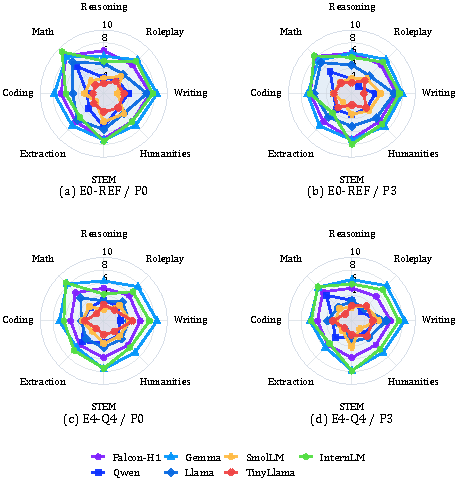
\includegraphics[width=0.49\textwidth,height=0.5\textwidth]{Figures/fig5_mtbench_category_radar_2x2_family.pdf}
    \caption{MT-Bench category scores by model family across eight open-ended capability categories.}
    \label{fig:mtbench-category-radar}
\end{figure}
\subsection{RQ4: What Do Falcon-H1 Results Tell Us?}
\label{sec:open-ended-results}

MT-Bench evaluates open-ended multi-turn instruction following with a
GPT-4o-mini judge and is therefore reported separately from reference-scored
correctness. Figure~\ref{fig:mtbench-category-radar} summarizes category-level
performance under the two extreme prompt and edge settings, while
Table~\ref{tab:mtbench-model} reports model-level MT-Bench scores.

Falcon-H1 is our primary study family because it is a recent SSM-hybrid SLM
line with multiple sub-4B variants. The results show strong matched-scale
instruction following: Falcon-H1-1.5B reaches 8.20 on MT-Bench, compared with
4.06 for Qwen2.5-1.5B at the same nominal scale. However, PEEL does not support
an architecture-exclusive robustness claim. Some dense Transformer families,
including Gemma and Phi, are also stable under prompt degradation when they are
well instruction-tuned. The more careful conclusion is that Falcon-H1 is a
strong matched-scale SLM family, while prompt robustness tracks post-training
quality and task format more than architecture alone.

\begin{table}[t]
\centering
\small
\setlength{\tabcolsep}{4pt}
\renewcommand{\arraystretch}{0.92}

\begin{tabular}{@{}lcccc@{}}
\toprule
Model & E0/P0 & E0/P3 & $\bar{E}$/P0 & $\bar{E}$/P3 \\
\midrule
FH1-90M        & 5.30 & 5.45 & 4.75 & 4.77 \\
FH1-0.5B       & 7.67 & 7.29 & 7.72 & 7.37 \\
FH1-0.6B       & 5.14 & 4.74 & 3.45 & 3.10 \\
FH1-1.5B       & \textbf{8.20} & 8.28 & 8.08 & 8.20 \\
FH1-1.5B-D     & 8.21 & 8.20 & 8.22 & 8.21 \\
Qwen-0.5B      & 3.39 & 2.88 & 3.05 & 3.08 \\
Qwen-1.5B      & \textbf{4.06} & 3.49 & 4.17 & 3.60 \\
Gemma-1B       & 7.42 & 7.28 & 7.40 & 7.28 \\
Llama-1B       & 7.00 & 6.72 & 4.55 & 4.16 \\
Llama-3B       & 3.92 & 4.22 & 4.10 & 3.89 \\
Phi-3.5M       & 8.20 & 8.16 & 5.74 & 5.73 \\
Phi-4M         & 7.51 & 7.69 & 5.57 & 5.66 \\
SmolLM-360M    & 2.81 & 2.73 & 2.68 & 2.76 \\
SmolLM-1.7B    & 3.45 & 3.45 & 3.50 & 3.04 \\
TinyLlama-1.1B & 2.42 & 2.48 & 2.55 & 2.49 \\
InternLM-1.8B  & 2.53   & 2.41   & 6.78 & 6.69 \\
\bottomrule
\end{tabular}
\caption{Model-level MT-Bench scores using GPT-4o-mini as judge. $\bar{E}$ averages over edge settings; Falcon-H1-1.5B scores 8.20 vs.\ Qwen2.5-1.5B 4.06 at E0/P0.}

\label{tab:mtbench-model}
\end{table}

Table~\ref{tab:mtbench-model} also shows that some strong E0/P0 scores
(Phi-3.5-mini 8.20, Llama-1B 7.00) fall sharply once averaged over edge
settings, because \texttt{llama.cpp} does not apply their chat template under
GGUF; Falcon-H1-1.5B, by contrast, is stable across the edge ladder. At the same time, PEEL does
not support an architecture-exclusive robustness claim. InternLM and Gemma show
the strongest overall family-level performance across categories, and some
dense Transformer families are similarly stable under prompt degradation. The
more careful conclusion is therefore that Falcon-H1 is a strong matched-scale
SLM family, while prompt robustness tracks instruction-tuning quality and task
format more than architecture alone.



\subsection{RQ5: What Should Practitioners Take Away?}
\label{sec:safety-results}

For practitioners, clean benchmark accuracy is not a sufficient deployment
signal. The preceding results show three separate risks: runtime changes under
edge deployment, prompt-contract collapse on short-answer tasks, and
task-dependent robustness on multiple-choice, rule-based, and open-ended
evaluations. Safety adds another interface-level concern: refusal behavior may
change even when task accuracy appears stable. HarmBench attack success rate
(ASR) is better when lower, XSTest safe over-refusal is better when lower, and
XSTest unsafe refusal is better when higher. Table~\ref{tab:safety-overall-heatmap}
reports these metrics across E0--E4 and P0/P3.


\begin{table}[t]
\centering

\begin{tabular}{m{20mm}lccccc}
\toprule
Metric & Prompt & E0 & E1 & E2 & E3 & E4 \\
\midrule
\multirow{2}{24mm}{HarmBench ASR}
& P0 & \cellcolor[HTML]{F4CCCC}21.7 & \cellcolor[HTML]{F4CCCC}21.7 & \cellcolor[HTML]{F9DDCC}21.3 & \cellcolor[HTML]{E6EDD1}20.2 & \cellcolor[HTML]{FDF2CC}20.7 \\
& P3 & \cellcolor[HTML]{E3ECD1}20.1 & \cellcolor[HTML]{FFF1CC}20.8 & \cellcolor[HTML]{E4ECD1}20.1 & \cellcolor[HTML]{EAEED0}20.3 & \cellcolor[HTML]{D9EAD3}19.9 \\\midrule
\addlinespace[1pt]

\multirow{2}{24mm}{XSTest safe over-refusal}
& P0 & \cellcolor[HTML]{F4CCCC}55.4 & \cellcolor[HTML]{FEEECC}54.3 & \cellcolor[HTML]{F9DCCC}54.9 & \cellcolor[HTML]{FEEDCC}54.4 & \cellcolor[HTML]{FFF2CC}54.2 \\
& P3 & \cellcolor[HTML]{FFF2CC}54.2 & \cellcolor[HTML]{E6EDD1}53.4 & \cellcolor[HTML]{EAEED0}53.5 & \cellcolor[HTML]{ECEED0}53.6 & \cellcolor[HTML]{D9EAD3}53.0 \\\midrule
\addlinespace[1pt]

\multirow{2}{24mm}{XSTest unsafe refusal}
& P0 & \cellcolor[HTML]{F5CFCC}73.4 & \cellcolor[HTML]{F4CCCC}73.2 & \cellcolor[HTML]{FBE6CC}74.6 & \cellcolor[HTML]{FBE6CC}74.6 & \cellcolor[HTML]{F9DDCC}74.1 \\
& P3 & \cellcolor[HTML]{FEF0CC}75.2 & \cellcolor[HTML]{F7D7CC}73.8 & \cellcolor[HTML]{D9EAD3}77.4 & \cellcolor[HTML]{E2ECD1}76.9 & \cellcolor[HTML]{FBE6CC}74.6 \\
\bottomrule
\end{tabular}
\caption{Overall rule-based safety metrics. Lower is better for HarmBench ASR and safe over-refusal; higher is better for unsafe refusal.}
\label{tab:safety-overall-heatmap}
\end{table}

The aggregate safety metrics remain relatively stable across edge settings.
Compared with P0, P3 yields slightly lower HarmBench ASR and safe over-refusal,
together with slightly higher unsafe refusal. However, these aggregate
differences are small and may conceal substantial variation across models. We
therefore treat the safety suite as a coarse diagnostic rather than a
model-level safety ranking. HarmBench and XSTest are retained as separate
metrics because improved harmful-request refusal may coincide with greater
refusal of benign prompts. The broader takeaway is that edge SLMs should be
evaluated as deployed systems: the failure mode may be prompt-contract
collapse, runtime-interface mismatch, instruction-tuning weakness, or refusal
instability, depending on the task.
\section{Conclusion}
\label{sec:conclusion}

We introduced PEEL, a benchmark for probing SLM performance along two real-world degradation axes: edge deployment and prompt quality. Across 1,088 reference-scored runs and 156 MT-Bench judge-scored runs, four findings emerge: (1) task format strongly determines robustness---short-answer tasks collapse under informal prompts, while multiple-choice tasks are less uniformly fragile; (2) Falcon-H1-1.5B substantially outperforms the matched-scale Qwen2.5-1.5B baseline on MT-Bench instruction following (8.20 vs.\ 4.06), while prompt robustness is not architecture-exclusive; (3) runtime and scoring artifacts can masquerade as capability collapse unless evaluation handles stop tokens, prompt echoes, and related interface artifacts; and (4) keyword-based safety diagnostics suggest non-trivial unsafe compliance, with ASR around 20--21\%, but should be treated as coarse refusal diagnostics rather than full safety evaluations. The Falcon-H1 case study suggests that edge-oriented SLMs should optimize not only clean instruction-following and efficiency, but also robustness to prompt degradation, runtime-interface variation, and refusal instability. We release prompts, evaluation scripts, and model outputs to support reproducibility and future lower-bound benchmarking.


\bibliography{references}



\end{document}
